\documentclass[10pt, a4paper]{article}
\usepackage{helvet}
\renewcommand{\familydefault}{\sfdefault}
\usepackage[english]{babel}
\usepackage[utf8x]{inputenc}
% package for including graphics with figure-environment
\usepackage{graphicx}
\usepackage{hyperref}
\usepackage{subcaption}
% colors for hyperlinks
% colored borders (false) colored text (true)
\hypersetup{colorlinks=true,citecolor=black,filecolor=black,linkcolor=black,urlcolor=black}

% package for bibliography
\usepackage[authoryear,round]{natbib}
% package for header
\usepackage[automark,headsepline]{scrlayer-scrpage}
\pagestyle{scrheadings}
\ihead[]{Text Detection in Natural Scene Images}
\ohead[]{September 30, 2021}
\cfoot[]{\pagemark} 

\begin{document}
	\title{
	\begin{figure}[!ht]
		% \flushleft
			
\includegraphics[width=0.26\textwidth]{img/htwlogo.jpg}
	\end{figure}
	\vspace{1cm}
	\Huge Text Detection in Natural Scene Images \\
	using EAST
	}
	
	\vspace{1cm}
	
	% if you are the only author, you might use the following
	% \author{Name of student}	
	
	% Insert here your name and correct mail address
	\author{\Large \href{mailto:s0566146@htw-berlin.de}{Henry Febrian}
	\vspace{1cm}}
	
	% name of the course and module
	\date{
	\large Module: \textit{Computergrafik und Bildverarbeitung} \\
	\vspace{0.8cm}
	\large Lecturer: Erik Rodner \\
	\vspace{1cm}
	\large September 30, 2021
	}

	\maketitle
	\setlength{\parindent}{0pt}

\vspace{2cm}
\begin{abstract}
To be edited at a later date. 

\end{abstract}
	\newpage
	\tableofcontents
	\newpage
	
\section{Introduction} % (fold)
\label{sec:introduction}
Text is arguably one of the most essential form of communication. Along with verbal communication, text is another reliable and effective medium to convey information in order for it to be understood. In this sense, text constitutes the cornerstone of human civilization \citep{LongEtAl}.
In the modern world, text is not only consumed by humans but has claimed its place in the world of technology.
However, text detection in natural scene images is proven to be challenging. Compared to detecting text on handwritten materials, the randomness of a natural scene is a big hurdle to overcome.

This paper aims to test and evaluate EAST on its performance in detecting natural-scene texts. 
EAST is chosen for its speed, efficiency, and accuracy on detecting text. It is widely available in OpenCV without complicated installation and implementation procedure.
The paper begins by observing the interference found on natural scenes followed by introducing and giving an overview of EAST.
It then provides an explanation of the evaluation dataset. Subsequently, the performance review of the algorithm will be presented, which is obtained by testing it on the aforementioned dataset.
% section introduction (end)

\section{Challenges of Natural Text Detection} % (fold)
\label{sec:challenges}
Natural scene images could be classified as images which are taken in uncontrolled environments, with any device ranging from smartphones to professional cameras. These images are snapshots of things in the real world.
\begin{figure}[h!]
	\centering
	\begin{subfigure}[b]{0.4\linewidth}
	  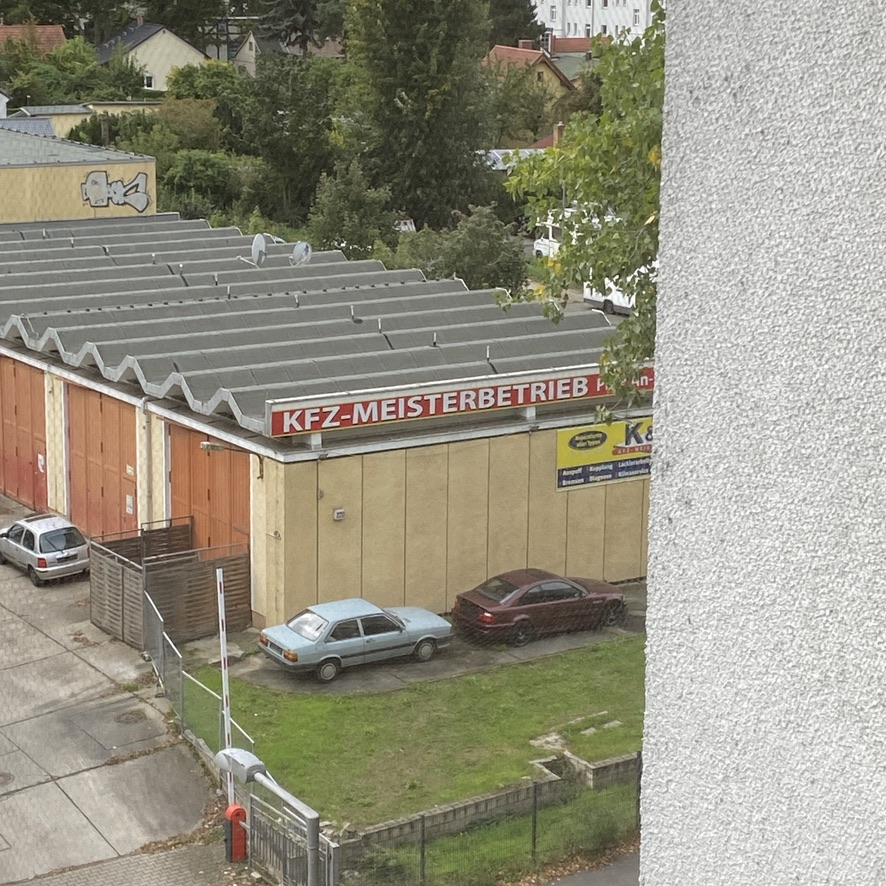
\includegraphics[width=\linewidth]{img/sample2.jpeg}
	  \caption{A scenery}
	\end{subfigure}
	\begin{subfigure}[b]{0.4\linewidth}
		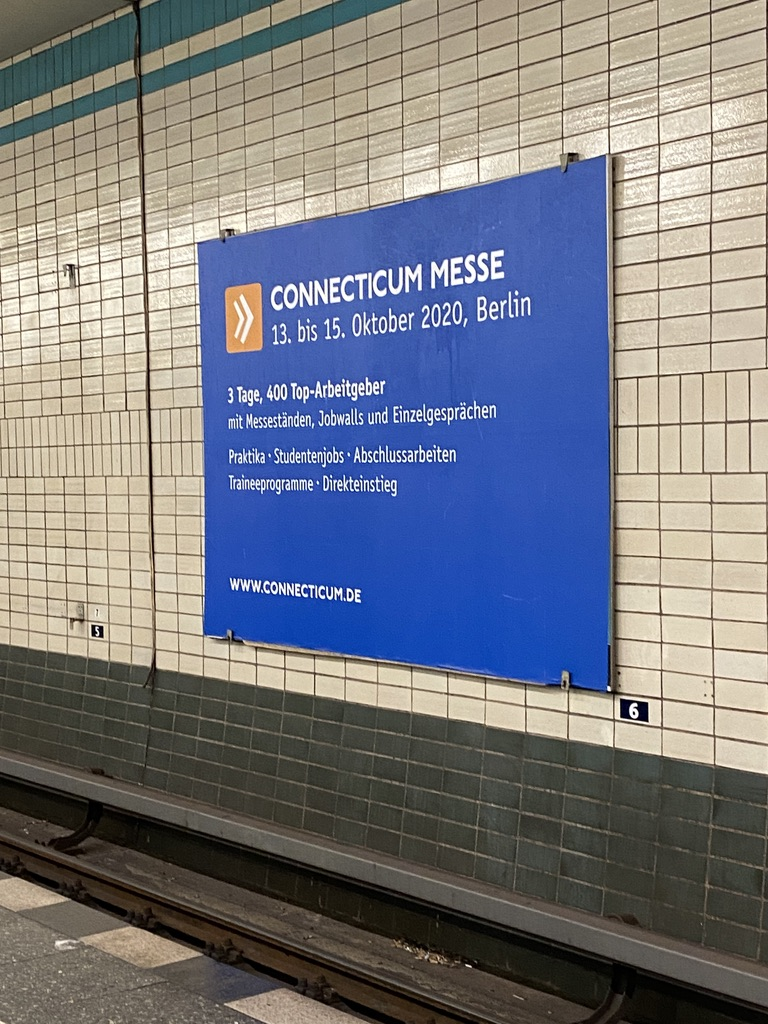
\includegraphics[width=\linewidth]{img/sample3.jpeg}
		\caption{A billboard}
	  \end{subfigure}
	\caption{Samples of natural scene images.}
	\label{fig:samples}
  \end{figure}

The random nature of the real world, combined with the diversity of available devices introduced some factors which make natural text detection a greater challenge than detecting structured text in documents. \cite{NaturalScene} mentioned some conditions that are found in natural scene which may significiantly impact text detection procedure. They are:
\begin{itemize}
	\item Raw sensor image and sensor noise
	\item Viewing angle
	\item Blur
	\item Lighting
	\item Resolution
	\item Non-paper objects
	\item Non-planar objects
\end{itemize}
Although devices have evolved to a point where most of handheld devices are capable of shooting in a high resolution, low-end handheld cameras and older models still struggle in this sector.
Uncontrolled environment, combined with the possible lack of stabilization from the equipment can cause blur \citep{Rosebrockeast}. Also, there are countless factors such as the time of the day, weather, camera flash, and many others which may impact the lighting conditions, further hindering the ability to detect text. Non-paper objects such as glass and plastic may reflect images, and non-planar objects such as text wrapped around a bottle becomes distorted and deformed \citep{Rosebrockeast}.
Additionally, there might be patterns that are extremely similar to text, or occlusions caused by foreign objects, which may potentially lead to confusion and mistakes \citep{LongEtAl}.
% section challenges (end)

\clearpage

\section{Methodology} % (fold)
\label{sec:methodology}
\subsection{Overview of EAST} % (fold)
\label{sub:overvieweast}
According to \cite{EastZhouEtAl}, the key component of EAST is a neural network model, which is trained to directly predict the existence of text instances and their geometries from full images \citep{EastZhouEtAl}.
Hence, the abbreviation EAST: Efficient and Accurate Scene Text Detector.
\begin{figure}[hbt!]
	\centering
	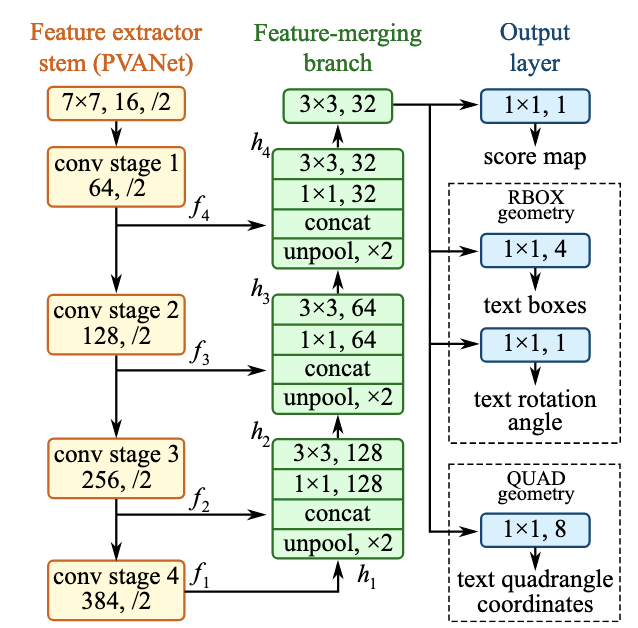
\includegraphics[width=0.5\textwidth]{img/eaststructure.png}
	\caption{Schematic view of EAST, adopted from Figure 3 of~\protect\cite{EastZhouEtAl}}
	\label{fig:east1}
\end{figure}

As claimed by \cite{EastZhouEtAl}, EAST is among the most efficient text detectors that achieve state-of-the-art performance on benchmarks.
The idea of the network is adopted from U-shape (or U-net) \citep{unet}, which simultaneously merges the feature maps and keeps the upsampling branches small. 

The end result is a network which is able to utilize different levels of features while keeping the computation cost low \citep{EastZhouEtAl}.
It is capable of predicting text on 720p images, running at an average of 13 FPS. The fastest setting, which reached a speed of 16.8 FPS was achieved on a combination of their algorithm with PVANET on 720p images using NVIDIA Titan X graphics card. \citep{EastZhouEtAl}.

The network undergoes and end-to-end training using ADAM \citep{adam} optimizer. 512x512 crops from images are uniformly sampled to form a minibatch of size 24 to accelerate the learning process.
Learning rate of ADAM starts from 1e-3, decays to one-tenth every 27300 minibatches, and stops at 1e-5. The network is trained until performance stops improving \citep{EastZhouEtAl}.
% subsection overvieweast (end)

\clearpage

\subsection{Testing} % (fold)
\label{sub:testing}
The test will be done on three different data groups with varying degrees of difficulties. They will be divided into easy, intermediate, and hard. The aim of this test is to see how the method performs on detecting text in natural scene images, determined by the detection rate and speed.

The grouping criteria of the dataset are as follow: the 'easy' group consists of images which are not natural scene. These are scanned images from item packaging and books.
\begin{figure}[hbt!]
	\centering
	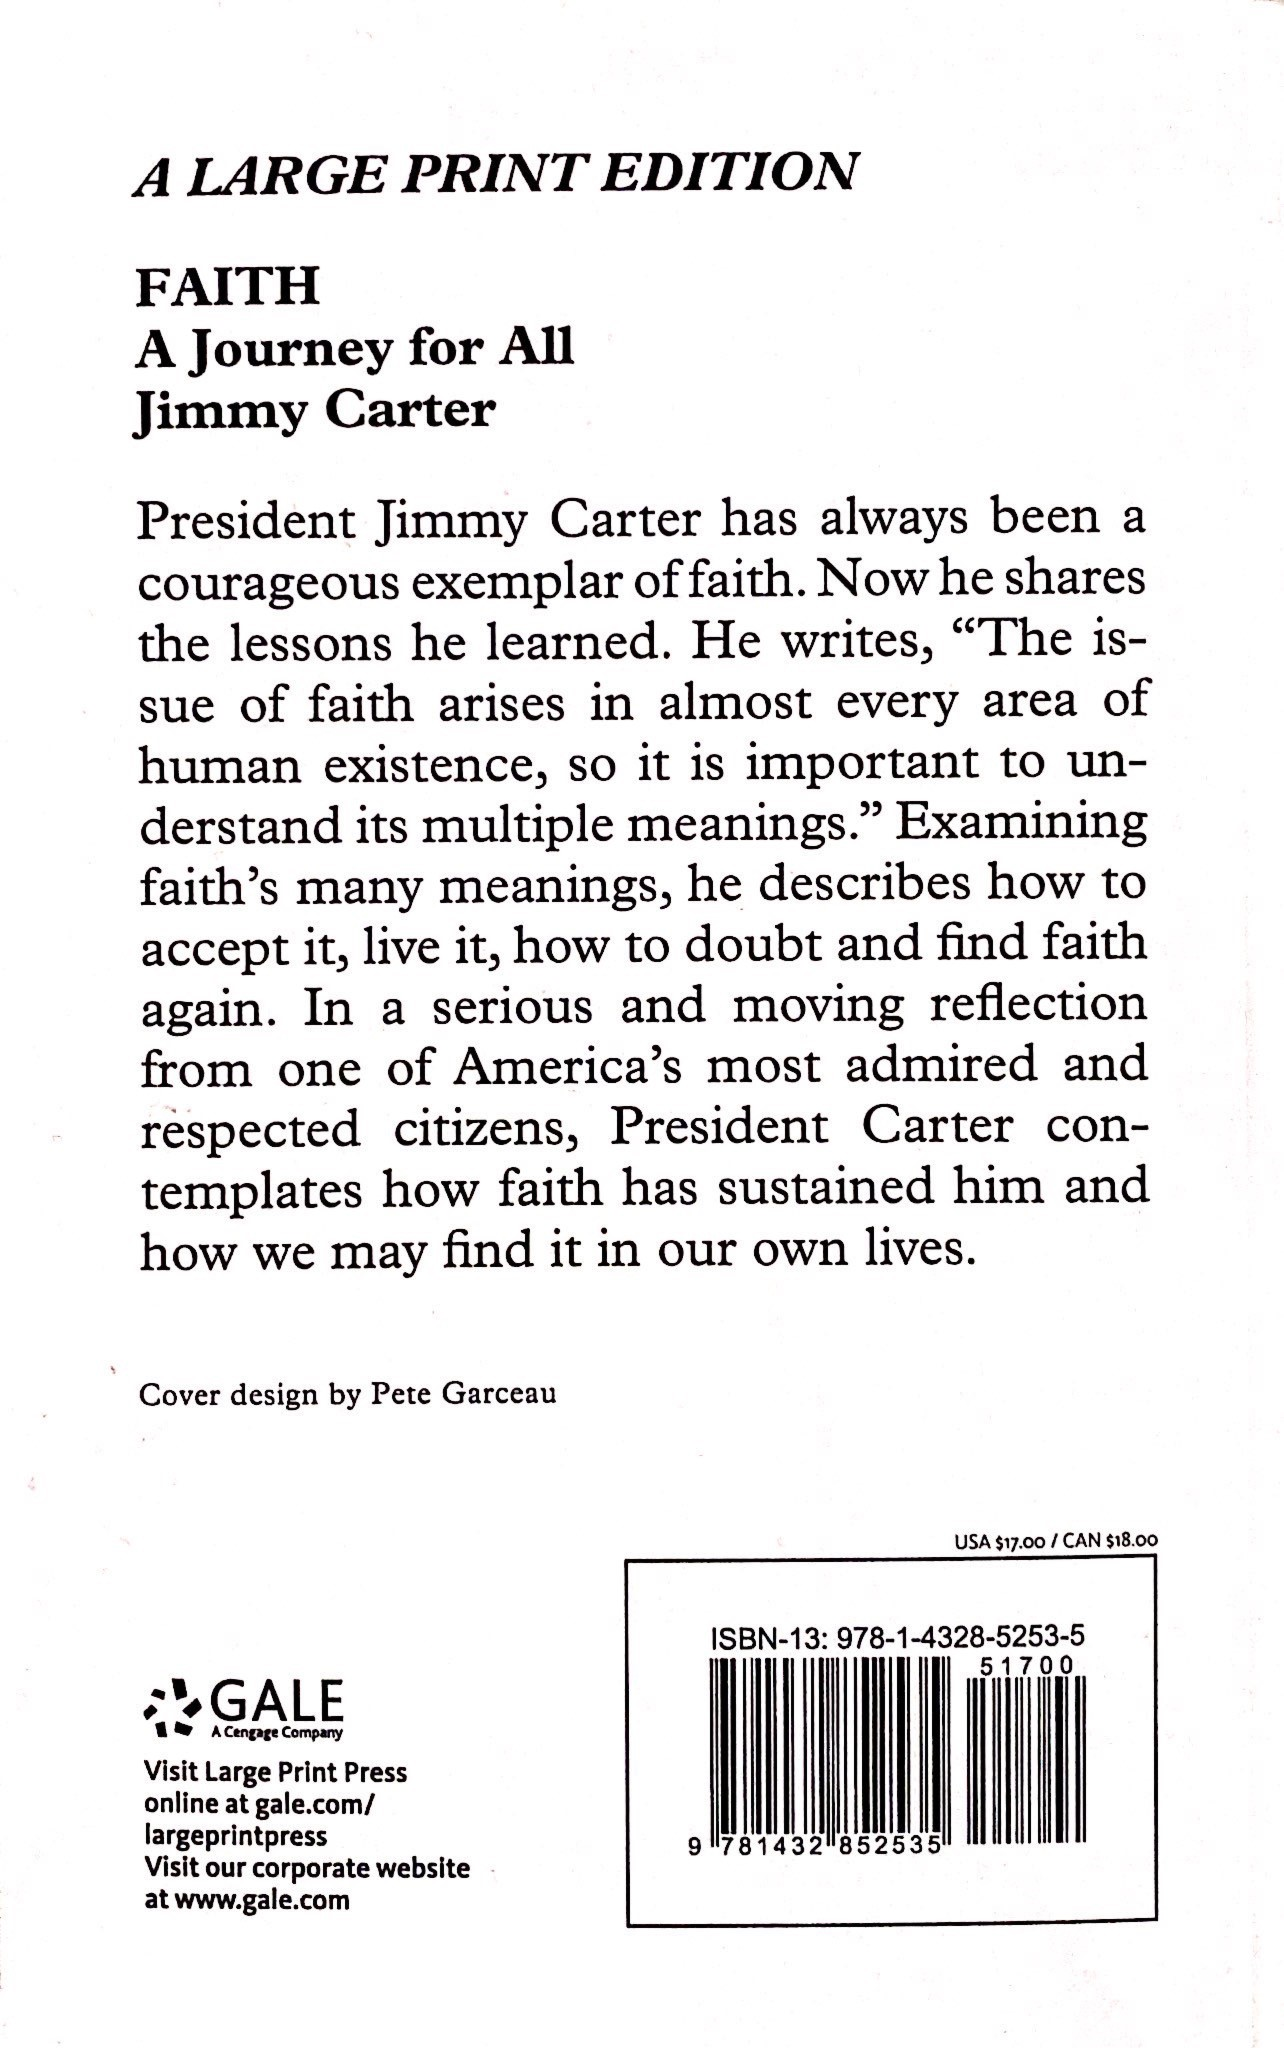
\includegraphics[width=0.5\textwidth]{img/sampleeasy.JPG}
	\caption{A sample image from the 'easy' group}
	\label{fig:sampleeasy}
\end{figure}

The 'intermediate' group is classified as such because it contains natural scene images which are taken relatively close to the camera with optimal lighting conditions and one obstructing factor from the following:
\begin{itemize}
	\item Condensed, small texts
	\item Mirroring effects
	\item Movement
	\item Object is far from the camera
	\item Old camera effect
	\item Poor lighting conditions
	\item Text is obstructed behind something else
	\item Wrapped text / distorted text
\end{itemize}

The 'hard' group consists of natural scene images with two or more of the aforementioned factors.
\begin{figure}[h!]
	\centering
	\begin{subfigure}[b]{0.4\linewidth}
		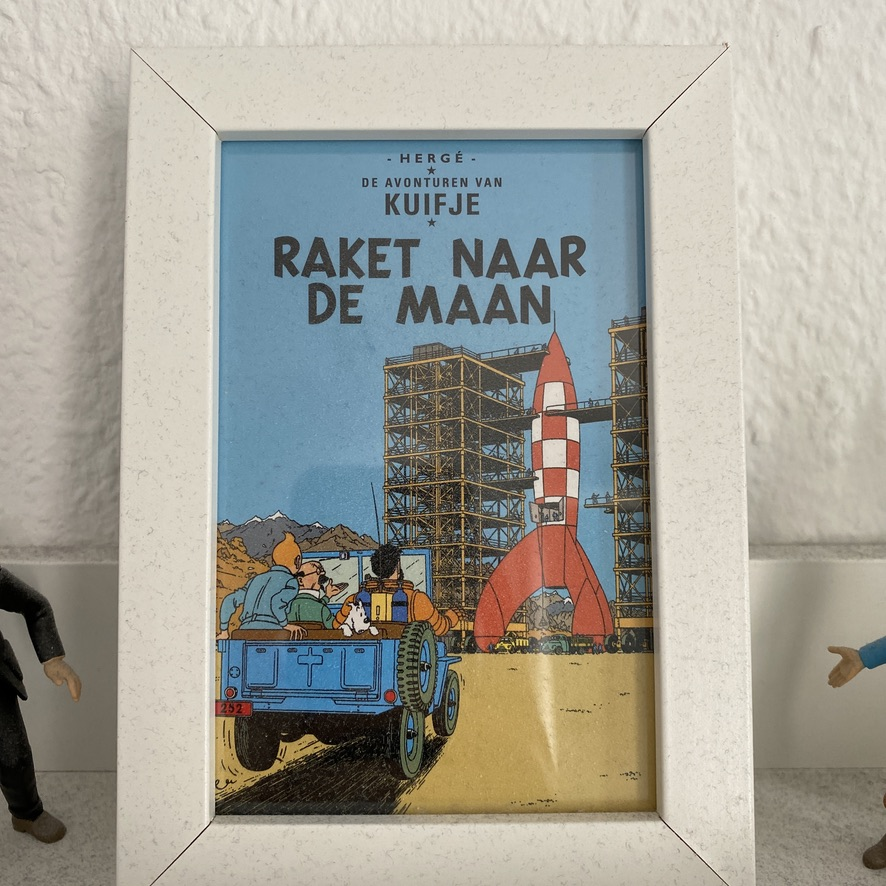
\includegraphics[width=\linewidth]{img/sample1.jpeg}
		\caption{A sample image from the 'intermediate' group}
	\end{subfigure}
	\begin{subfigure}[b]{0.4\linewidth}
		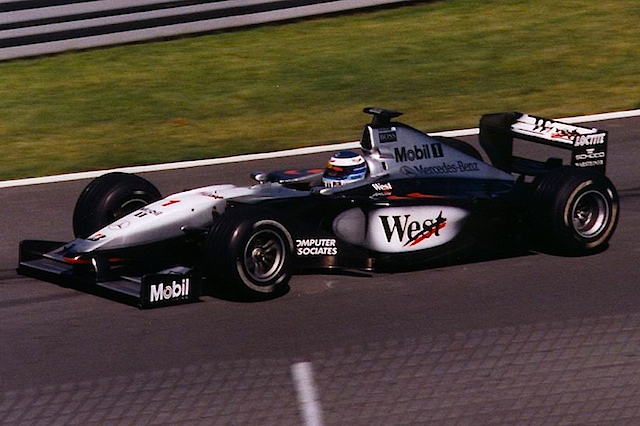
\includegraphics[width=\linewidth]{img/samplehard.JPG}
		\caption{A sample image from the 'hard' group, from \cite{mikapic}}
	\end{subfigure}
	\caption{Samples of image from intermediate and hard dataset group.}
	\label{fig:samples_dataset}
  \end{figure}

Each dataset group contains approximately six images with similar criteria, which are grouped in their own folders. The network will run through each dataset group and the total time that it needs to detect everything will be presented in the following chapter.

The results will be saved as a separate image which can be eyeballed 

% subsection testing (end)
% section methodology (end)
\clearpage
\section{Results and Evaluation} % (fold)
\label{sec:evaluation}
tba
% section evaluation (end)

\section{Conclusion} % (fold)
\label{sec:conclusion}
tba
% section conclusion (end)
\clearpage
\newpage 

\bibliographystyle{natdin}
	\bibliography{references} % expects file "references.bib"
	\addcontentsline{toc}{section}{References}
\end{document}